\section{Основные понятия теории моделирования}

\begin{figure}[H]
    \centering
    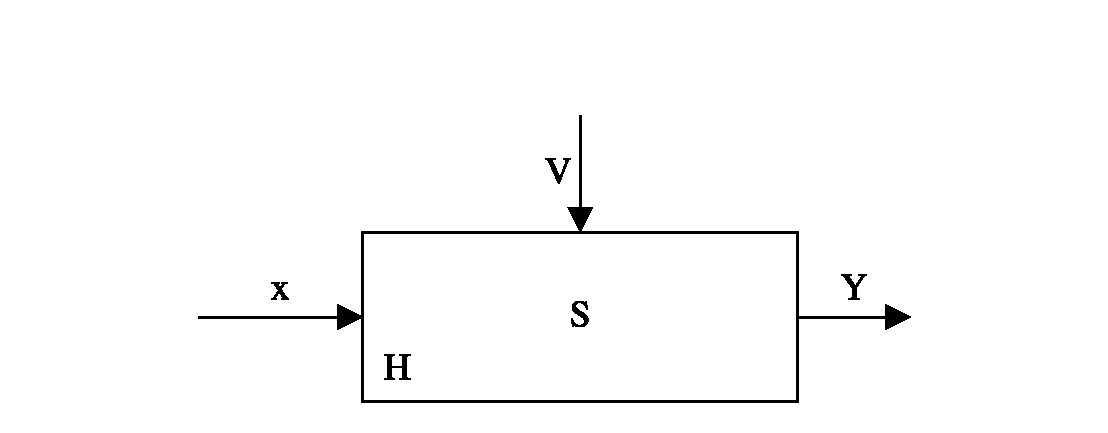
\includegraphics[width=0.8\textwidth]{img/content/05_general_modeling/scheme.pdf}
    \caption{Модель объекта}
    \label{fig:scheme}
\end{figure}

Модель объекта можно представить в виде множества величин, описывающих функционирование реальной системы и образующих в лучшем случае следующие подмножества:

\begin{enumerate}
    \item Совокупность входных воздействий на систему $x_i \in X, i = \overline{1, n_X}$
    \item Совокупность воздействия внешней среды $v_l \in V, j = \overline{1, n_V}$
    \item Совокупность внутренних собственных параметров системы $h_k \in H, k = \overline{1, n_H}$
    \item Совокупность выходных характеристик системы $y_j \in Y, j = \overline{1, n_Y}$
\end{enumerate}

В общем случае они являются элементами непересекающихся подмножетсв и содержат в себе как детерминированные, так и стахостатические состовляющие. При анализе функционирования системы $S$ входные воздействия, воздействия внешней среды и внутренние параметры являются независимыми (экзогенными). Которые имеют следующий вид

\begin{equation*}
    \vec x(t) = \left( x_1(t), x_2(t), \ldots, x_{n_X}(t) \right)
\end{equation*}

\begin{equation*}
    \vec v(t) = \left( v_1(t), v_2(t), \ldots, v_{n_V}(t) \right)
\end{equation*}

\begin{equation*}
    \vec h(t) = \left( h_1(t), h_2(t), \ldots, h_{n_H}(t) \right)
\end{equation*}

А выходные характеристики являются зависимыми (эндогенными)

\begin{equation*}
    \vec y(t) = \left( y_1(t), y_2(t), \ldots, y_{n_Y}(t) \right)
\end{equation*}

Процесс функционирования системы $S$ описывается во времени некоторым оператором, который преобразует независимые переменные в зависимые в соотвествии с соотношением

\begin{equation*}
    \vec y (t) = F_S (\vec x, \vec v, \vec h, t )
\end{equation*}

Эта зависимость называется \textbf{законом функционирвоания системы}. В общем случае он может быть задан в виде функции, функционала, логриечских условий, в алгоримическом или табличном видах и т.д.

Очень важным являеся понятие \textbf{алгоритма функционирования системы} ($A_S$). Под \textbf{алгоритмом} будем подразуемевать метод получения выходных характеристик с учетом входных воздействий, воздействий внешней среды и соответствующих параметров системы. Закон функционирования может быть получен и через свойства системы. В конкретные моменты времени называемыми \textbf{состяниями}.

\begin{equation*}
    \vec z (t) = \left( z_1 (t), z_2(t), \ldots, z_{n_z}(t) \right)
\end{equation*}

Если рассматривать как последовательную смену состояний, то они могут быть интерпретированы как координаты точки в $k$-мерном пространстве. Причем каждой реализации процесса будет соответствовать некоторая фазовая траектория. Совокупность всех состяний системы на интервале от 0 до $t$ называется \textbf{пространством состояний}.

Состояние системы в некоторый момент $t_v \le t \le t_V$ полностью определяется некоторыми начальными условиями, входными воздействиями, внутренними параметрами, воздействиями внешней среды с помощью следующих уравнений

\begin{equation*}
    \begin{cases}
        \vec z (t) = \Phi ( \vec z^o, \vec x, \vec v, \vec h, t) \\
        \vec y(t) = F(\vec z, t) \\
    \end{cases}
\end{equation*}

\begin{equation*}
    \vec y(t) = F(\Phi ( \vec z^o, \vec x, \vec v, \vec h, t), t)
\end{equation*}

Следовательно, под математической моделью реальной системы понимаем конечное множество переменных вместе с математическими связями между ними и характеристиками выходными.
